\chapter{Examples of useful LaTeX features and writing hints} 
\label{cha:hints}

\section{Citations}
\label{sec:citations}
This is an example citation \cite{WaBo2016}. This is another example citation \cite{wallscheid2014real}. You can also combine them as \cite{WaBo2016,wallscheid2014real}. This is done via the \verb|\cite{}| command. This command is used to reference a source in the text. The source is then automatically listed in the bibliography at the end of the document. The bibliography is created using the \href{https://ctan.org/pkg/biblatex}{biblatex} package. The \texttt{references.bib} file is a BibTeX file. BibTeX is a reference management software for formatting lists of references. It is widely used in academia for this purpose, and it is also used in the \LaTeX\ document preparation system.

Some general hints on citations:
\begin{itemize}
	\item Use quotation marks only for direct quotes from a primary source. If you refer to a general statement, idea or observation of a source, do not use quotation marks but rather paraphrase the content and add a citation at the end of the sentence.
	\item Also add citation marks to figures, tables, etc. if they are not your own work or if you have adapted them from another source.
	\item Always ensure that the citation is correct and that the source is reliable, that is, stick to peer-reviewed scientific journals, conference proceedings, books, etc. and avoid using non-reviewed sources such as blogs or general websites.
\end{itemize}



\section{Upper and lower case formatting}
\label{sec:formatting}
 In titles and captions, capitalize only the beginning of the sentence. In the main text, capitalize the first letter of the first word of a sentence. Hence, stick to lower case formatting as the default representation. In contrast, proper nouns need to be capitalized whenever used (e.g, ``Maxwell's equations'' or ``Kalman filter''). Note that technical terms are not necessarily proper nouns and should not be capitalized (e.g., ``state-space model'' or ``convolutional neural network''). Also, when introducing abbreviations, there is no need to capitalize the full term (e.g., ``recurrent neural network (RNN)'').

\section{Tables}
\label{sec:features}
In \tabref{tab:params} some arbitrary dummy parameters are summarized for demonstration purpose. The table is created using the \href{https://ctan.org/pkg/booktabs}{booktabs} package.
\begin{table}[htb]
	\caption{Considered input and target parameters.}
	\label{tab:params}
	\centering
	\begin{tabular}{l c c}
		\toprule
		Parameter name & Symbol & Model position \\
		\midrule
		Ambient temperature & $\vartheta_\mathrm{a}$ & Input \\
		Actual voltage $d$-axis component & $u_\mathrm{d}$ & Input \\
		Actual voltage $q$-axis component & $u_\mathrm{q}$ & Input \\
		Actual current $d$-axis component & $i_\mathrm{d}$ & Input \\
		Actual current $q$-axis component & $i_\mathrm{q}$ & Input \\
		\hline
		Permanent magnet temperature & $\vartheta_{\mathrm{PM}}$ & Output \\
		Stator teeth temperature & $\vartheta_{\mathrm{ST}}$ & Output \\
		Stator winding temperature & $\vartheta_{\mathrm{SW}}$ & Output \\
		Stator yoke temperature & $\vartheta_{\mathrm{SY}}$ & Output\\
		\bottomrule
	 \end{tabular}
\end{table}

 It is considered good style to use only horizontal lines for the top, bottom and between table body sections while avoiding vertical lines. This is because vertical lines are considered to be less readable and less aesthetic. The table is also centered and has a caption. The caption is placed above the table (while figures' captions are typically placed below the figure, compare \figref{fig:cnn}). This is a common style convention in scientific writing. 



\section{Mathematical typesetting}
\label{subsec:normalization}
This is an in-text equation example: $T(t)=3/2\psi_{\mathrm{PM}}i_{\mathrm{q}}(t)$. After this equation, we can continue writing normal text. A simple intended equation is
\begin{equation}
	\label{eq:example}
	\frac{\mathrm{d}}{\mathrm{d}t}x(t) = f(x(t),u(t),t),
\end{equation}
where $x(t)\in\mathbb{R}$ is the state, $u(t)\in\mathbb{R}$ is the input, $f(\cdot)\in\mathbb{R}\rightarrow\mathbb{R}$ represents the state dynamics and $t\in\left[0,T\right]$ is the time. In this scalar equation, all variables are represented in regular font. If any variable or parameter of an equation is of vectorial / matrix / multidimensional nature (e.g., $\bm{x}(t)\in\mathbb{R}^n$), it should be represented in bold font. For example,
\begin{equation*}
	\bm{x}(t) = \bm{A}\bm{x}(t) + \bm{b}u(t)
\end{equation*}
represents a linear time-invariant state-space example of  \eqref{eq:example}, where $\bm{A}\in\mathbb{R}^{n\times n}$ is the state matrix, $\bm{b}\in\mathbb{R}^{n}$ is the input vector and $u(t)\in\mathbb{R}$ is the input vector (which is the only non-bold symbol in the above equation due to its scalar nature). Note also that the last example equation is not numbered which is achieved by using the \verb|\begin{equation*}|...\verb|\end{equation*}| environment. Discontinuing the numbering of an equation can be useful when the equation is not referred to in the text and if it is of minor importance.

Using the \verb|\eqref{}| command one can directly refer to a labeled equation. For example, \eqref{eq:example} is a simple example of a first-order ordinary differential equation. Within the STEM community it is good practice to refer to equations in the parenthesis style (e.g., ``...as shown in \eqref{eq:example}''), that is, the parenthesis is already indicating an explicit reference to an equation making the usage of the word ``equation'' redundant. 


Equations can also be aligned and split:
\begin{align}
    a&=b+c,\\
    \begin{split}
        \frac{\mathrm{d}}{\mathrm{d}t}x_2(t)&= \frac{1}{C_2} \left( i_1(t)-i_2(t)\right)= \frac{1}{C_2} \left[ \frac{1}{R_1} \left(u(t)-x_2(t)-x_1(t) \right)-\frac{1}{R_2} x_2(t)\right]\\
        &= \frac{1}{C_2 R_1} u(t)-\frac{1}{C_2 R_1} x_1(t) - \frac{1}{C_2} \left( \frac{1}{R_1}+\frac{1}{R_2}\right) x_2(t). 
        \label{eq:splitline}
    \end{split}
\end{align}

In \eqref{eq:splitline} the equation was split into two lines. Use this for long equations. Note also that the above equations are integrated in the text and reading flow which includes proper interpunctuation, that is, full stops and commas apply also to equations as if they would be normal text.

Note: Using variables, the variable itself should be in italic letters, while any superscript or subscript should be in upright letters (unless it is a mathematical variable, e.g., a counting index such as $x_i$ with $i=1,2,\ldots$). Hence, $x_\mathrm{norm}(t)$ is correct, while $x_{norm}(t)$ is not. Likewise, mathematical operators (e.g., differential operator, transpose, etc.) are generally represented in upright letters, that is, $\max\left\{x_\mathrm{norm}(t)\right\}$ is correct, while $max \left\{x_{\mathrm{norm}}(t) \right\}$ is not.

 \section{Units}
 \label{sec:units}
 In engineering, it is important to use the correct units. For example, the speed of light is $c = \SI{299792458}{\meter\per\second}$. The unit of the speed of light is $\si{\meter\per\second}$.
 
 This is called a quantity equation (also called complete equation), where the unit of measurement and the physical unit are explicitly separated to represent a physical quantity. When using a quantity equation, ensure sticking to the International System of Units (SI units). This requires to display SI units in upright letters and in roman font. The numerical number is separated from the SI unit by a space. The easiest way to achieve this is by using the \href{https://ctan.org/pkg/siunitx}{siunitx} package.    

\section{Figures}
\label{sec:architecture}
In \figref{fig:cnn} is an example how to insert figures into the manuscript. Please note that figures should be always integrated as vector graphics (e.g., PDF, EPS, SVG) and not as pixel-based raster graphics (e.g., PNG, JPEG). This is to ensure that the figures are crystal clear and require minimum file size.\footnote{There are only very few and rare exceptions to this rule. Besides photographs (e.g., of laboratory setups) figures covering an excessive amount of data content, such as scatter plots with thousands of data points (slowing down the vector graphic representation), can be mentioned as such exceptions. And by the way: this is an example of a footnote which can be used to place comments or small excursions at the bottom of a page.} Hence, ensure that you are preparing your explanatory graphics in a vector-based software (e.g., Inkscape) and also export figures prepared in Matlab, Python, Julia, etc. in a suitable vector format. 

\begin{figure}[htb]
	\centering
    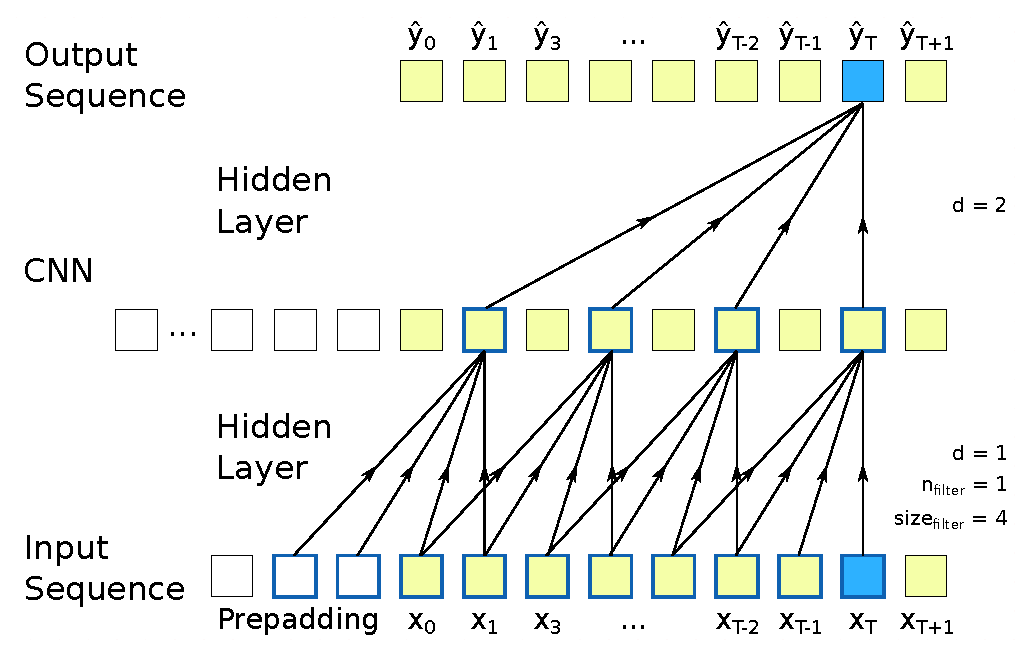
\includegraphics[width=0.75\textwidth]{modeling/CNN_over_sequence.eps}
    \caption{Examaple of a convolutional neural network.}
	\label{fig:cnn}
\end{figure}

\section{Acronyms and glossaries}
\label{sec:acronyms}
This is an example of an acronym entry: \gls{chp}. The first time an acronym is used, it is spelled out in full and the acronym is placed in brackets. The acronym is then automatically added to the list of acronyms at the end of the document. The list of acronyms is created using the \href{https://ctan.org/pkg/glossaries}{glossaries} package. The \texttt{glossaries.tex} file is used to define the acronyms. Starting the second time an acronym is used, only the short acronym form is used, such as \gls{chp}.

This is an example of a glossary entry: \gls{CHPg}. The glossary is different from the acronyms as it lists terms together with a short definition for those terms (with the glossary list at the end of the document). A glossary is sometimes used in larger books or theses to explain terms that are not commonly known, but for most scientific theses or papers it is rather uncommon to use a glossary. 

